%%%%%%%%%%%%%%%%%%%%%%%%%%%%%%%%%%%%%%%%%
% Structured General Purpose Assignment
% LaTeX Template
%
% This template has been downloaded from:
% http://www.latextemplates.com
%
% Original author:
% Ted Pavlic (http://www.tedpavlic.com)
%
% Note:
% The \lipsum[#] commands throughout this template generate dummy text
% to fill the template out. These commands should all be removed when 
% writing assignment content.
%
%%%%%%%%%%%%%%%%%%%%%%%%%%%%%%%%%%%%%%%%%

%----------------------------------------------------------------------------------------
%	PACKAGES AND OTHER DOCUMENT CONFIGURATIONS
%----------------------------------------------------------------------------------------

\documentclass{article}

\usepackage{fancyhdr} % Required for custom headers
\usepackage{lastpage} % Required to determine the last page for the footer
\usepackage{extramarks} % Required for headers and footers
\usepackage{graphicx} % Required to insert images
\usepackage{lipsum} % Used for inserting dummy 'Lorem ipsum' text into the template

% Margins
\topmargin=-0.45in
\evensidemargin=0in
\oddsidemargin=0in
\textwidth=6.5in
\textheight=9.0in
\headsep=0.25in 

\linespread{1.1} % Line spacing

% Set up the header and footer
\pagestyle{fancy}
\lhead{\hmwkAuthorName} % Top left header
% \chead{\hmwkClass\ ( \hmwkClassInstructor\ \hmwkClassTime): \hmwkTitle} % Top center header
\rhead{\firstxmark} % Top right header
\lfoot{\lastxmark} % Bottom left footer
\cfoot{} % Bottom center footer
\rfoot{Page\ \thepage\ of\ \pageref{LastPage}} % Bottom right footer
\renewcommand\headrulewidth{0.4pt} % Size of the header rule
\renewcommand\footrulewidth{0.4pt} % Size of the footer rule

\setlength\parindent{0pt} % Removes all indentation from paragraphs

%----------------------------------------------------------------------------------------
%	DOCUMENT STRUCTURE COMMANDS
%	Skip this unless you know what you're doing
%----------------------------------------------------------------------------------------

% Header and footer for when a page split occurs within a problem environment
\newcommand{\enterProblemHeader}[1]{
\nobreak\extramarks{#1}{#1 continued on next page\ldots}\nobreak
\nobreak\extramarks{#1 (continued)}{#1 continued on next page\ldots}\nobreak
}

% Header and footer for when a page split occurs between problem environments
\newcommand{\exitProblemHeader}[1]{
\nobreak\extramarks{#1 (continued)}{#1 continued on next page\ldots}\nobreak
\nobreak\extramarks{#1}{}\nobreak
}

\setcounter{secnumdepth}{0} % Removes default section numbers
\newcounter{homeworkProblemCounter} % Creates a counter to keep track of the number of problems

\newcommand{\homeworkProblemName}{}
\newenvironment{homeworkProblem}[1][Reviewer \arabic{homeworkProblemCounter}]{ % Makes a new environment called homeworkProblem which takes 1 argument (custom name) but the default is "Problem #"
\stepcounter{homeworkProblemCounter} % Increase counter for number of problems
\renewcommand{\homeworkProblemName}{#1} % Assign \homeworkProblemName the name of the problem
\section{\homeworkProblemName} % Make a section in the document with the custom problem count
\enterProblemHeader{\homeworkProblemName} % Header and footer within the environment
}{
\exitProblemHeader{\homeworkProblemName} % Header and footer after the environment
}

\newcommand{\problemAnswer}[1]{ % Defines the problem answer command with the content as the only argument
\noindent\framebox[\columnwidth][c]{\begin{minipage}{0.98\columnwidth}#1\end{minipage}} % Makes the box around the problem answer and puts the content inside
}

\newcommand{\homeworkSectionName}{}
\newenvironment{homeworkSection}[1]{ % New environment for sections within homework problems, takes 1 argument - the name of the section
\renewcommand{\homeworkSectionName}{#1} % Assign \homeworkSectionName to the name of the section from the environment argument
\subsection{\homeworkSectionName} % Make a subsection with the custom name of the subsection
\enterProblemHeader{\homeworkProblemName\ [\homeworkSectionName]} % Header and footer within the environment
}{
\enterProblemHeader{\homeworkProblemName} % Header and footer after the environment
}
   
%----------------------------------------------------------------------------------------
%	NAME AND CLASS SECTION
%----------------------------------------------------------------------------------------

\newcommand{\hmwkTitle}{Reviewer Comments Answer} % Assignment title
\newcommand{\hmwkDueDate}{Wednesday,\ January\ 28,\ 2015} % Due date
\newcommand{\hmwkClass}{} % Course/class
\newcommand{\hmwkClassTime}{} % Class/lecture time
\newcommand{\hmwkClassInstructor}{} % Teacher/lecturer
\newcommand{\hmwkAuthorName}{Dynamic Rendezvous based Routing Algorithm on Sparse Opportunistic Network Environment: IJDSN/819178.v1 : Jiradett Kerdsri and Komwut Wipusitwarakun} % Your name

%---------------------------------------------------------------------------------------
%	TITLE PAGE
%----------------------------------------------------------------------------------------

\title{
\vspace{2in}
\textmd{\textbf{\hmwkClass:\ \hmwkTitle}}\\
\normalsize\vspace{0.1in}\small{Due\ on\ \hmwkDueDate}\\
\vspace{0.1in}\large{\textit{\hmwkClassInstructor\ \hmwkClassTime}}
\vspace{3in}
}

\author{\textbf{\hmwkAuthorName}}
\date{} % Insert date here if you want it to appear below your name

%----------------------------------------------------------------------------------------

\begin{document}

% \maketitle

%----------------------------------------------------------------------------------------
%	TABLE OF CONTENTS
%----------------------------------------------------------------------------------------

%\setcounter{tocdepth}{1} % Uncomment this line if you don't want subsections listed in the ToC

% \newpage
% \tableofcontents
% \newpage

%----------------------------------------------------------------------------------------
%	Reviewer1
%----------------------------------------------------------------------------------------

% To have just one problem per page, simply put a \clearpage after each problem

\begin{homeworkProblem} 
The authors introduce the concept of rendezvous place where the passing nodes can announce, deposit or pickup their own messages without having to meet the other nodes carrying the desired message. 
%%
In the proposed scheme, the rendezvous place is detected automatically and its area’s size and shape are dynamically changed according to the interaction among nodes passing around the area. 
%%
The results from simulations show that their proposed routing algorithm can achieve higher delivery ratio and utilize lower energy consumption than original opportunistic routing algorithms especially in sparse network environment.

It is true that by introducing the several mechanisms, the authors’ proposal can achieve the performance in terms of the packet delivery ratio and energy consumption. 
%%

\begin{homeworkSection}{[Question 1]} % Section within problem
However, is the opportunistic routing actually applicable in the real situation? 
%%
The delivery ratio of 90\% or less is quite insufficient, it is worse that the delivery ratio is much dependent on the network parameters. 
%%
It may be the reviewer’s personal opinion. 
%%
Thus, the authors should clearly state the actual application scenarios of the proposed method. 

\problemAnswer{ % Answer

}
\end{homeworkSection}
%----------------------------------------------------------------------------------------

\begin{homeworkSection}{[Question 2]} % Section within problem
In the paper, the authors refer to the wildlife monitoring. 
%%
If it is one application that they suppose, they should consider the simulation model based on it. 
%%
The reviewer’s feeling is that the simulation model is too generic, and the readers could not have a confidence that the proposed method is useful. 
%%
The same argument can be applied to the predictable behavior of OppNet nodes. 
%%
Its applicability must be heavily dependent on the target system.
%%
Perhaps a more realistic realization is to use mobile robots to collect information around the field. 
%%
Even in the sparse environment, the path planning method can make the delivery ratio of packets higher. 
%%
See the related papers.

\problemAnswer{ % Answer

}
\end{homeworkSection}
%----------------------------------------------------------------------------------------

\begin{homeworkSection}{[Question 3]} % Section within problem
In summary, for the paper to be accepted, the authors clearly describe the application of the proposed method, and show the simulation results based on the application scenarios. Also, they should discuss why the proposed method is better than the other methods including the planning method using the mobile robots.

\problemAnswer{ % Answer

}
\end{homeworkSection}

\end{homeworkProblem}

\clearpage
%----------------------------------------------------------------------------------------
%	Reviewer2
%----------------------------------------------------------------------------------------


\begin{homeworkProblem}

This manuscript proposed a concept of rendezvous place for improving delivery ratio and reducing energy consumption in sparse opportunistic networks. 
%%
But some details are still unclear.
%----------------------------------------------------------------------------------------

\begin{homeworkSection}{[Question 1]} % Section within problem
How long could a message stay in the Rendezvous node buffer, if the Rendezvous node didn't encounter the target node? 

\problemAnswer{ % Answer
In the opportunistic network environments, a message is commonly embedded with a time-to-live (TTL) parameter (or called a message deadline) which stops the packets from traveling unnecessarily throughout the network \cite{Prodhan2011,Yuan2012,Nguyen2009,Khabbaz2012}. 
%
Our provious work \cite{Kerdsri2013} has shown that the different value of message deadlines can affect the delivery ratio. 
%
In our design, each message will be dropped once it reach the message deadline in order to clear the messages left on the buffer of Rendezvous node.
%%
If the capacity of data storage in Rendezvous node is fully occupied, then the oldest messages will be dropped once the new messages arrives.
%%
In our simulation, we setup the TTL to the simulation time in order to hold the messages in the Rendezvous zone as long as possible.
%%
We assume that Rendezvous buffer is large enough to feasible store as many messages waiting to pickup by target nodes.
%%
Therefore, the messages will indefinitely stay in the Rendezvous node buffer until the storage is full and the newer messages request the space from the buffer.
}
\end{homeworkSection}
%----------------------------------------------------------------------------------------

\begin{homeworkSection}{[Question 2]} % Section within problem
If the Rendezvous node can't find the expected node-gathering area for a long time, does it keep moving? In this process, is it broadcasting the Rendezvous Area rumor message (RA)? 

\problemAnswer{ % Answer
In our system, the Rendezvous node will move to a new location if there is insufficient contact from OppNet node within a predefined duration.
%
Consequently,the Rendezvous node will situate in the node-gathering area when there is enough number of encountered OppNet nodes.
%%
Therefore, the Rendezvous nodes will keep moving until they meet the desired conditions.
%%
In addition, in the process of moving, the Rendezvous node will keep broadcasting the Rendezvous Area rumor message ($RA$), so the OppNet nodes can learn that they are in the Rendezvous zone when they detect the $RA$ messages. 
}
\end{homeworkSection}
%----------------------------------------------------------------------------------------

\begin{homeworkSection}{[Question 3]} % Section within problem
Moreover, how does it determine its center location when implementing sweeping algorithm? How do you see the relationship between the period of sweep mechanism and the period of searching Rendezvous place?

\begin{figure}[h]
\centering
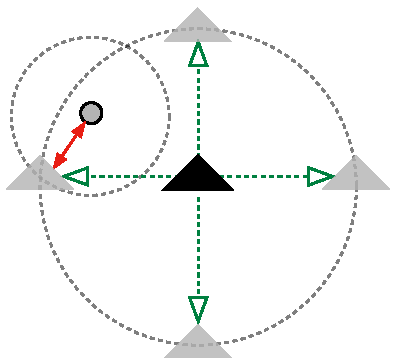
\includegraphics[width=1.5in]{Figures/Sweep.pdf}
\caption{Sweep mechanism}
\label{Sweep mechanism}
\end{figure}

\problemAnswer{ % Answer
The sweeping mechanism is started when the Rendezvous node station in the desire location in order to gain more delivery ratio from the nodes with different transmission range.
%%
The center location of Rendezvous for the sweeping algorithm is determined by its radio range since the Rendezvous node can move to 4 direction as in Fig. \ref{Sweep mechanism}.
%%
The period of sweep mechanism and searching Rendezvous place are irrelevant since the sweeping always performs when the Rendezvous node is stationed while the period of searching is depended on the encountered OppNet nodes.
}
\end{homeworkSection}
%----------------------------------------------------------------------------------------

\begin{homeworkSection}{[Question 4]} % Section within problem
The Rendezvous node should passively wait for the target node entering the Rendezvous place. Does it harm the efficiency of packet delivery, compared with some latest opportunistic routings?

\problemAnswer{ % Answer
}
\end{homeworkSection}
%----------------------------------------------------------------------------------------

\begin{homeworkSection}{[Question 5]} % Section within problem
Furthermore, some of the references in the section 2 are too old. And author should choose at least one recent opportunistic routing protocol for comparison in the evaluation.

\problemAnswer{ % Answer
}
\end{homeworkSection}

\end{homeworkProblem}

%%%%%%%%%%%%%%%%%%%
%     References
%%%%%%%%%%%%%%%%%%%

\bibliographystyle{abbrv}
\bibliography{refs}


\end{document}
